\section{\RU{Мусор в стеке}\EN{Noise in stack}}

\RU{Часто в этой книге я говорю о ``шуме'' или ``мусоре'' в стеке или памяти.}
\EN{Often in this book I write about ``noise'' or ``garbage'' values in stack or memory.}
\RU{Откуда он берется}\EN{Where do they come from}?
\RU{Это то, что осталось там после исполнения предыдущих функций.}
\EN{These are what was left in there after other functions' executions.}
\RU{Короткий пример}\EN{Short example}:

\lstinputlisting{patterns/02_stack/08_noise/st.c}

\RU{Компилируем}\EN{Compiling}\dots

\lstinputlisting[caption=\NonOptimizing MSVC 2010]{patterns/02_stack/08_noise/st.asm}

\RU{Компилятор поворчит немного}\EN{The compiler will grumble a little bit}\dots

\begin{lstlisting}
c:\Polygon\c>cl st.c /Fast.asm /MD
Microsoft (R) 32-bit C/C++ Optimizing Compiler Version 16.00.40219.01 for 80x86
Copyright (C) Microsoft Corporation.  All rights reserved.

st.c
c:\polygon\c\st.c(11) : warning C4700: uninitialized local variable 'c' used
c:\polygon\c\st.c(11) : warning C4700: uninitialized local variable 'b' used
c:\polygon\c\st.c(11) : warning C4700: uninitialized local variable 'a' used
Microsoft (R) Incremental Linker Version 10.00.40219.01
Copyright (C) Microsoft Corporation.  All rights reserved.

/out:st.exe
st.obj
\end{lstlisting}

\RU{Но когда я запускаю}\EN{But when I run the compiled program}\dots

\begin{lstlisting}
c:\Polygon\c>st
1, 2, 3
\end{lstlisting}

\RU{Ох. Вот это странно. Мы ведь не устанавливали значения никаких переменных в}\EN{Oh, 
what a weird thing! We did not set any variables in} \TT{f2()}. 
\RU{Эти значения --- это ``привидения'', которые всё ещё в стеке.}
\EN{These are ``ghosts'' values, which are still in the stack.}

\clearpage
\RU{Загрузим пример в}\EN{Let's load the example into} \olly:

\begin{figure}[H]
\centering
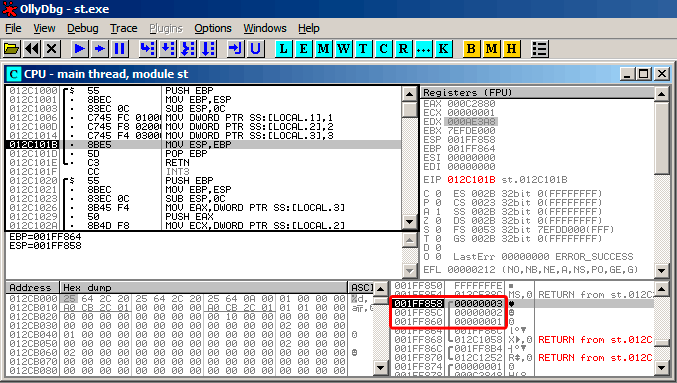
\includegraphics[scale=\FigScale]{patterns/02_stack/08_noise/olly1.png}
\caption{\olly: \TT{f1()}}
\label{fig:stack_noise_olly1}
\end{figure}

\RU{Когда}\EN{When} \TT{f1()} \RU{заполняет переменные}\EN{assigns the variables} $a$, $b$ \AndENRU $c$ 
\RU{они сохраняются по адресу}\EN{, their values are stored at the address} \TT{0x14F860} 
\RU{и т.д.}\EN{and so on.}

\clearpage
\RU{А когда исполняется}\EN{And when} \TT{f2()}\EN{ executes}:

\begin{figure}[H]
\centering
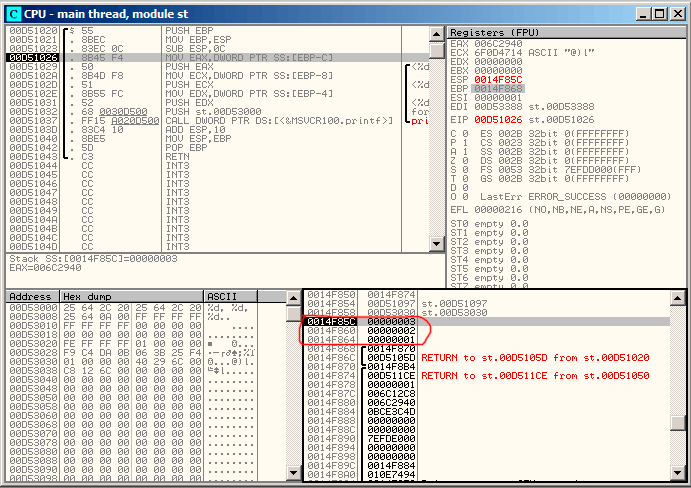
\includegraphics[scale=\FigScale]{patterns/02_stack/08_noise/olly2.png}
\caption{\olly: \TT{f2()}}
\label{fig:stack_noise_olly2}
\end{figure}

... $a$, $b$ \AndENRU $c$ \RU{в ф-ции}\EN{of} \TT{f2()} \RU{находятся по тем же адресам!}
\EN{are located at the same addresses!}
\RU{Пока никто не перезаписал их, так что они здесь в нетронутом виде.}
\EN{No one has overwritten the values yet, so at that point they are still untouched.}

\RU{Для создания такой странной ситуации несколько функций должны исполняться друг за другом
и \ac{SP} должен быть одинаковым при входе в функции, т.е., у функций должно быть равное количество
аргументов). Тогда локальные переменные будут расположены в том же месте стека.}
\EN{So, for this weird situation, several functions has to be called one after another and
\ac{SP} has to be the same at each function entry (i.e., they  has same number
of arguments). Then the local variables will be located at the same positions in the stack.}

\RU{Подводя итоги, все значения в стеке (да и памяти вообще) это значения оставшиеся от 
исполнения предыдущих функций.}
\EN{Summarizing, all values in the stack (and memory cells in general) 
have values left there from previous function executions.}
\RU{Строго говоря, они не случайны, они скорее непредсказуемы.}
\EN{They are not random in the strict sense, but rather have unpredictable values.}

\RU{А как иначе}\EN{Is there other option}?
\RU{Можно было бы очищать части стека перед исполнением каждой функции,
но это слишком много лишней (и ненужной) работы.}
\EN{It probably would be possible to clear portions of the stack before each function execution,
but that's too much extra (and unnecessary) work.}
